\section{Benchmark Findings}

\textbf{Evidence tiers.} Headline controlled and provenance results use the one-time 5,000-cluster paper test. Separately frozen tests cover 500 powered Binance dates and 200 dates with \RealAgentProposalRows{} actual-model proposals. MES is descriptive; event-market, cross-generator, and learner analyses are prospective validation evidence. All community-hidden partitions remain unevaluated.

\subsection{Finding 1: Coverage collapse makes low NUAR insufficient}
Table~\ref{tab:main_results} reports the controlled paper test. Direct Prior authorizes every row (NUAR 0.656; ALR 0.250). Cost-Aware has the lowest NUAR, 0.064, but ALR 0.245 and certification volume zero. Lifecycle has NUAR 0.147, ALR zero, certification volume 0.30, coverage 0.293, and review rate 0.429. No Action has zero coverage and NUAR/ALR \textit{N/A}; it cannot win by abstaining everywhere.

The registered stress-to-ordinary coverage audit separates selective omission from uniformly low action rates. Cost-Aware has collapse index \CostAwareCollapseIndex{} and Lifecycle \LifecycleCollapseIndex{}, whereas Direct Prior and Hard Role Gate remain uniform. Thus low NUAR can coexist with materially narrower coverage on difficult profiles.

\begin{table*}[t]
  \caption{\textbf{Paper-test operating points and validation conservative hypervolume reject a single-winner interpretation.} CAU is cumulative authorized utility; MOC is missed opportunity cost; Val. HV is a pre-frozen validation sensitivity. Full certification grids and the Pareto set appear in the supplement. \textit{N/A} denotes structural zero authorization.}
  \label{tab:main_results}
  \centering
  \benchmarktableformat
  % Generated by finauth_audit/paper/generate_tables.py. Do not edit manually.
\begin{tabular}{lrrrrrrr}
\toprule
Rule & Cov. & NUAR & ALR & Review & CAU & MOC & Val. HV \\
\midrule
No Action & 0.000 & \textit{N/A} & \textit{N/A} & 0.000 & 0.00 & 31.20 & 0.000 \\
Direct Prior & 1.000 & 0.656 & 0.250 & 0.000 & 20.38 & 0.00 & 0.000 \\
Confidence Gate & 0.382 & 0.099 & 0.250 & 0.000 & 39.46 & 0.00 & 0.000 \\
Uncertainty Gate & 0.386 & 0.109 & 0.248 & 0.000 & 39.31 & 0.01 & 0.000 \\
Risk Filter & 0.635 & 0.610 & 0.209 & 0.000 & 23.31 & 5.97 & 0.036 \\
Cost-Aware Gate & 0.367 & 0.064 & 0.245 & 0.000 & 40.77 & 0.01 & 0.003 \\
Hard Role Gate & 0.750 & 0.656 & 0.000 & 0.000 & 16.01 & 0.00 & 0.209 \\
Lifecycle Checklist & 0.293 & 0.147 & 0.000 & 0.429 & 30.14 & 0.63 & 0.195 \\
\bottomrule
\end{tabular}

\end{table*}

Validation-to-paper-test rank correlations are effectively 1.000, but frozen policy profiles and continuous hypervolume select different operating points; seven nonzero-action rules lie on the exact four-dimensional Pareto set. \textbf{Finding 1: FinAuth-Audit exposes a multi-objective authorization frontier; low NUAR is neither necessary nor sufficient for a valid comparison.}

\subsection{Finding 2: Clean current roles do not prevent lineage laundering}
Figure~\ref{fig:provenance} and Table~\ref{tab:provenance_results} report the provenance paper test. Hard Role Gate has zero direct leakage but ALR 0.172. Provenance Hard Gate reduces ALR to zero at coverage 0.591 and safe-delegation coverage 0.698; the learned gate raises coverage to 0.603 while accepting ALR 0.018. Low NUAR does not imply clean lineage: Lifecycle has NUAR 0.146 and ALR 0.165; EPV has NUAR 0.039 and ALR 0.169.

\begin{figure*}[t]
  \centering
  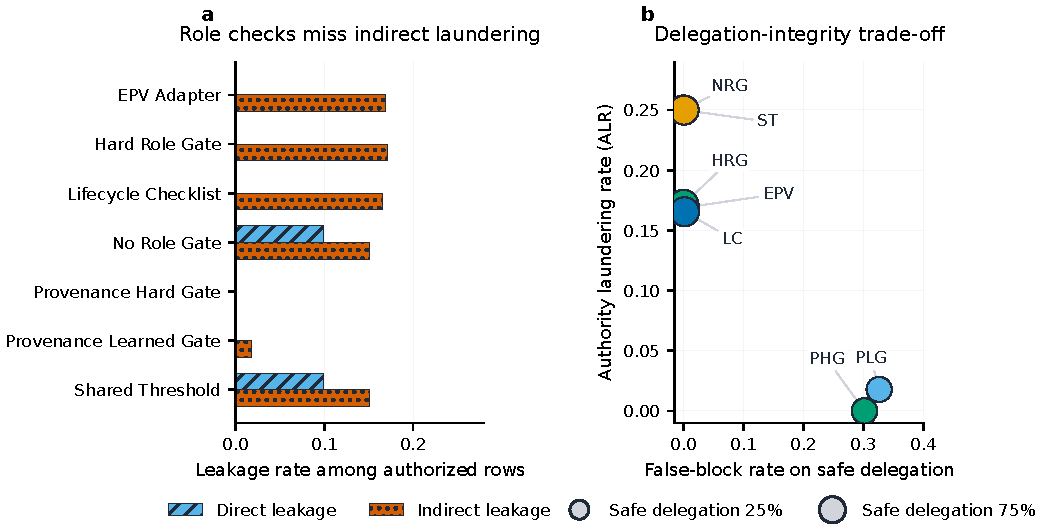
\includegraphics[width=\textwidth]{figures/fig_provenance_laundering.pdf}
  \Description{Two-panel paper-test provenance figure. The left panel compares direct and indirect leakage by rule. The right panel plots authority laundering rate against false-block rate on safe delegation.}
  \caption{\textbf{Current-role integrity, provenance integrity, and usable delegation differ on the paper test.} Panel (a) separates direct from indirect leakage using color and hatch. Panel (b) plots ALR against false blocking; bubble area encodes safe-delegation coverage. Labels abbreviate the rules listed in Table~\ref{tab:provenance_results}.}
  \label{fig:provenance}
\end{figure*}

\begin{table*}[t]
  \caption{\textbf{Paper-test provenance controls trade authorization quality, lineage integrity, delegation coverage, and review load.} Direct and indirect columns are leakage rates among authorized rows.}
  \label{tab:provenance_results}
  \centering
  \benchmarktableformat
  % Generated by finauth_audit/paper/generate_tables.py. Do not edit manually.
\begin{tabular}{lrrrrrrr}
\toprule
Rule & Cov. & FAR & ALR & Direct & Indirect & Safe del. & Review \\
\midrule
No Action & 0.000 & \textit{N/A} & \textit{N/A} & \textit{N/A} & \textit{N/A} & 0.000 & 0.000 \\
No Role Gate & 1.000 & 0.674 & 0.250 & 0.099 & 0.151 & 1.000 & 0.000 \\
Shared Threshold & 0.371 & 0.122 & 0.250 & 0.099 & 0.151 & 0.999 & 0.000 \\
Soft Penalty & 0.406 & 0.198 & 0.238 & 0.085 & 0.153 & 0.999 & 0.000 \\
Hard Role Gate & 0.879 & 0.674 & 0.172 & 0.000 & 0.172 & 1.000 & 0.121 \\
Provenance Hard Gate & 0.591 & 0.674 & 0.000 & 0.000 & 0.000 & 0.698 & 0.183 \\
Provenance Learned Gate & 0.603 & 0.668 & 0.018 & 0.000 & 0.018 & 0.674 & 0.100 \\
Lifecycle Checklist & 0.335 & 0.146 & 0.165 & 0.000 & 0.165 & 0.999 & 0.296 \\
EPV Adapter & 0.297 & 0.039 & 0.169 & 0.000 & 0.169 & 0.999 & 0.000 \\
\bottomrule
\end{tabular}

\end{table*}

The current-role-only Bayes risk is 0.129 on traceable rows and 0.256 on untraceable rows; legal partial signatures reduce it to 0.061 and 0.083. These registered-distribution values quantify ambiguity, not hidden-lineage recovery. \textbf{Finding 2: role eligibility and provenance integrity are distinct targets, and missing lineage creates an identifiable information cost.}

\subsection{Finding 3: The pilot inverse-transfer claim fails to reproduce}
The v0.6 paper test evaluates \RealAgentProposalRows{} cached proposals from three model configurations on two tasks across \RealAgentRankIndependentUnitCount{} independent UTC dates and five assets. The preregistered inverse-rank hypothesis is \RealAgentRankSupportStatus: Spearman $\rho=\RealAgentRankSpearman$, Kendall $\tau_b=\RealAgentRankKendall$, exact one-sided $p=\RealAgentRankExactP$, and bootstrap $\Pr(\rho<0)=\RealAgentRankNegativeProbability$. The binding result therefore retires the 60-date pilot estimate $\rho=-0.928$. Only \RealAgentPairwiseReversalCount{} of \RealAgentPairwiseComparisonCount{} pairs reverse; omitting Lifecycle gives $\rho=\RealAgentLifecycleOmitSpearman$. Nine malformed records remain deterministic non-action placeholders, and subgroup ranks remain diagnostic.

\begin{figure*}[t]
  \centering
  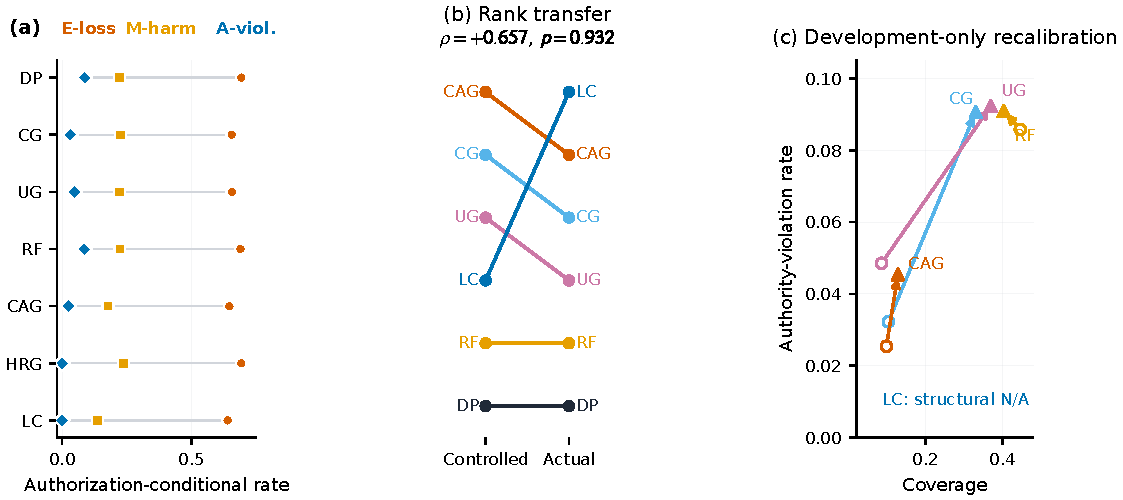
\includegraphics[width=\textwidth]{figures/fig_actual_model_validity.pdf}
  \Description{Three-panel actual-model paper-test figure. Panel a separates economic-loss, material-harm, and authority-violation rates by rule. Panel b compares controlled and actual-model economic-loss ranks. Panel c shows zero-shot to development-recalibrated movement in coverage and authority-violation rate.}
  \caption{\textbf{Actual-model evidence separates consequence semantics, rank transfer, and threshold transport.} Panel (a) distinguishes economic loss, material harm, and authority violation. Panel (b) retains the failed preregistered inverse-rank test. Panel (c) compares zero-shot circles with development-only triangles; Lifecycle is structural \textit{N/A} because no candidate met the coverage floor.}
  \label{fig:actual_model_validity}
\end{figure*}

Endpoint choice changes interpretation: economic loss ranges from 0.641 to 0.694, material harm from 0.138 to 0.238, and authority violation from zero to 0.088. Lifecycle minimizes material harm and authority violation but covers only 0.121. Recalibration raises Confidence and Uncertainty coverage to 0.331 and 0.370 while raising authority violation to 0.091 and 0.092; Lifecycle remains structural \textit{N/A}. Threshold adjustment is not a universal transport repair.

Validation-only mechanistic generators remain less stable against utility IID ($\rho=0.683$ and $0.738$) than against each other ($\rho=0.994$), and the sequential generator certifies no rule. \textbf{Finding 3: the benchmark retires an attractive pilot claim and reports localized sensitivity without replacing a failed primary with subgroups.}

\subsection{Finding 4: Validity gates retain mixed, underpowered, and undefined evidence}
The preregistered 500-date Binance IUT \textbf{fails} despite power 0.970/0.965. Cost-Aware minus Lifecycle passes the negative-utility arm ($-0.0170$, 95\% CI $[-0.0198,-0.0138]$), but laundering rises only $+0.0154$ ($[+0.0140,+0.0168]$), below its $+0.020$ SESOI. MES remains descriptive because its fixed bundle yields a non-estimand role contrast.

The event-market layer passes data-integrity checks but has power 0.164 (LCB95 0.160), below 0.80; it remains \emph{exploratory-only} and sealed.

The registered learner comparison is undefined because a held-out mechanism violates the 5\% coverage-LCB floor. At 20,000 clusters, full-audit and coverage-constrained selective Logistic recover five of six mechanisms, but sequential-market coverage still collapses; complete cross-mechanism NUAR remains \textit{N/A}. \textbf{Finding 4: validity gates retain powered mixed failure, underpowered transfer, and undefined learner evidence instead of converting them into wins.}

Supplementary Figure~\ref{fig:validity_gates} visualizes these unchanged statuses.
